% Chapter Template
\chapter{Solution Design} % Main chapter title
\label{Chapter3} % Change X to a consecutive number; for referencing this chapter elsewhere, use \ref{ChapterX}
\section{General Approach} \label{sec:generalApproach}

The objectives mentioned in section Sec.\ref{sec:thesisGoals} were achieved by following the workflow shown below in figure \ref{fig:workflow}. This workflow contains five stages: (1) Instrumentation of the applications, (2) Exploration, (3) Coverage measurement, (4) Summarize data, and (5)  Data Analysis. 

\begin{figure}[h]
\centering
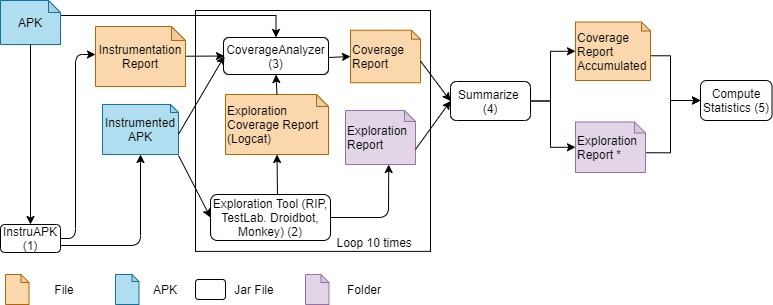
\includegraphics[width=\textwidth]{../Figures/workflow.jpg}
\caption{Main Workflow}\label{fig:workflow}
\end{figure}

For the first stage, \textbf{InstruAPK} (Section \ref{sec:instruAPK}) was used to make the instrumentation of the applications. This tool only takes into account the methods under the package name of the application that is being analysed. As a result, methods from different libraries are not instrumented. The input for this stage is the original APK file. The output is the instrumented APK, together with the instrumentation report containing general information such as the file path, method's name, file name, and the method arguments, as well as a sequential number that will help us to know the total amount of instrumented methods and will work as their unique identifier.

In the stage number two, the exploration was made with four different exploration tools, (1) Droidbot \ref{sec:droidbot}, (2) Monkey \footnote{https://developer.android.com/studio/test/monkey}, (3) Firebase Test Lab \ref{sec:testlab}, and (4) RIP \ref{sec:rip}. Every tool was executed to explore apps with a maximum time of 30 minutes. It is important to notice that, even when the max execution time seems to be short, it was enough for most of the analysed applications. This was because of the size of the applications: if the application is small, then the coverage will increase rapidly, because a bug was found during the exploration, or even because the tool marks the exploration as done. 

This stage input is only the instrumented APK file, and its output is the exploration report that every tool provides. Most of the time, the report contains the device logcat after the exploration. In the case of Monkey, it was extracted by using an adb command \footnote{https://developer.android.com/studio/command-line/logcat} because it is not extracted by the tool itself.

Droidbot, Monkey and Firebase Test Lab were selected because of their high use in the industry, and RIP was selected because it is an active project from The Software Design Lab. 

In stage 3, \textbf{CoverageAnalyzer (CA)} (Section \ref{sec:ca}) was used to make the coverage measurement and search for error lines. This stage inputs are the original APK, the instrumentation report and the instrumented APK, both from stage 1, and the logcat from stage 2. The output is a report containing two method coverage measurements, the first one, calculated using the number of methods reported by APKAnalyzer \footnote{https://developer.android.com/studio/command-line/apkanalyzer}, a tool provided in the Android SDK Tools, and the second one with the number of instrumented methods reported by InstruAPK.

Stages 2. and 3. were repeated ten times for every application that was selected. The multiple executions are intending to get average values as well as comparable results along with the different exploration tools. On top of that, input for stage 4 is all the method coverage reports form stage 3 as well as the exploration report from stage 2. The output is the accumulated method coverage by each tool for each application, which was calculated taking the unique methods called over all the ten executions, the average accumulated method coverage over time, as well as the number of errors and its average, found per application.

The final stage, i.e.,  Stage 5,  encompasses data understanding, graphs creation, a comparison using the graph and analysis of different qualitative aspects of every exploration tool. Providing the figures presented in chapter \ref{Chapter4}, as well as leading to the conclusions in chapter \ref{Chapter5} and helping to fulfil reach the objectives proposed at the beginning of this document.

\section{InstruAPK}\label{sec:instruAPK}

This tool \footnote{https://github.com/TheSoftwareDesignLab/InstruAPK} was developed for this study. It uses APKTool, a known Java application that allows inverse engineering of Android apps, allowing applications' instrumentation without the need of recompiling their source code. APKTool decodes the APK file and its result is the smali \footnote{https://github.com/JesusFreke/smali/wiki} representation of the app source code. These smali files are analysed in order to find all the methods to be instrumented at the very beginning of each method. It is important to notice that no external libraries methods are instrumented. InstruAPK only searches for methods following the android project structure that uses the application package name to store the application source code.

\begin{figure}[h]
\centering
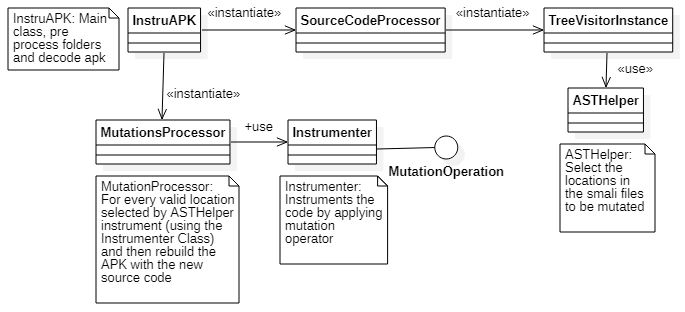
\includegraphics[width=0.8\textwidth]{../Figures/ClassDiagramInstruAPK.jpg}
\caption{Class Diagram InstruAPK}\label{fig:instruAPK}
\end{figure}

Figure \ref{fig:instruAPK} only contains the main classes of the tool and offers a short explanation of what is doing everyone to understand it in more detail.

\section{CoverageAnalyser (CA)}\label{sec:ca}

This tool \footnote{https://github.com/TheSoftwareDesignLab/CoverageAnalyzer} is a Java Application created for this study. It analyses the resulted logcat file after an exploration. It searches for the log lines injected by InstruAPK, as well as for errors, filtering the results using the package name of the application under the analysis. For the coverage measurement, the tool uses the number of methods reported by APKAnalyzer \footnote{https://developer.android.com/studio/command-line/apkanalyzer} as well as the number of methods reported by InstruAPK, resulting in two different method coverage values. As mentioned before, CA searches for the log lines injected by InstruAPK making CA depend on it. For that reason, CA can be seen as a complement of InstruAPK, rather than a separate application.

Figure \ref{fig:ca} contains the main classes of CoverageAnalyzer besides a short explanation of its functionality.

\begin{figure}[h]
\centering
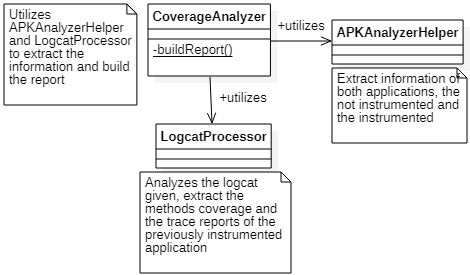
\includegraphics[width=0.8\textwidth]{../Figures/ClassDiagramCA.jpg}
\caption{Class Diagram Coverage Analyser}\label{fig:ca}
\end{figure}

These two tools are the main basis of this study, but its further review is left for previous studies. Both tools are now open source projects that can be found on Github.

Any person who desires to compare different exploration tools can reproduce this workflow. Even can make use of the same tools for the instrumentation and the coverage measurement, allowing easy and fast comparisons. Consequently, decision-making starts to be easier for developers and researchers. Also, gives the possibility to researchers to compare their exploration tools effortlessly and quickly.